\documentclass[11pt]{article}
\usepackage{geometry}
\geometry{
 a4paper,
 total={170mm,257mm},
 left=20mm,
 top=20mm,
 }
\usepackage[french]{babel}
\usepackage[T1]{fontenc}
\usepackage[utf8]{inputenc}
\usepackage{lmodern}
\usepackage{graphicx}
\usepackage{amssymb}
\usepackage{microtype}
\usepackage{hyperref}
\title{Petit état de l’art de la segmentation d’images par contours actifs}
\author{Raoelisolonarivony - MISA M2}
\date{Novembre 2016}

\begin{document}
\maketitle

\section{La segmentation}

Une image est formée de pixels. Le principe de la segmentation est de découper une image en composantes connexes ou régions constituées de pixels ayant une propriété commune: un niveau de gris proche ou une texture commune (par exemple la texture du bois).

Pour segmenter une image, une première approche est l'\textit{approche par régions}: il s'agit de regrouper les pixels similaires. Une autre approche est celle \textit{ par contours}: on s'intéresse aux frontières entre les régions, au changement brusque ou zone de rupture du critère de similarité pris en compte.

\section{La segmentation par contours actifs}

De nouvelles approches, les contours actifs, ont été introduites en 1987 et reposent sur des connaissances \textit{a priori} du contour: propriété de régularité et de continuité.
Un contour actif est un ensemble de points \textit{à priori} qu'on va tenter de déplacer pour lui faire épouser une forme.
C'est l'équipe Kass, Witkin et Terzopoulos \cite{snakes-active-contour-models} qui a travaillé en premier sur les contours actifs ou courbes minimisantes. Ce sont de courbes déformables comme des serpents d'où leur nom "snake".

A l'état initial de l'algorithme, le contour est disposé uniformément autour de l'objet à détecter puis il va se rétracter
pour en épouser au mieux les formes. De même, un contour actif peut aussi se dilater et essayer de remplir
un objet d'intérêt, il est placé à l'intérieur de cet objet à l'état initial dans ce cas.

\begin{figure}[!htbp]
\centering
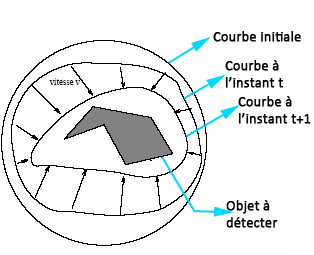
\includegraphics[width=6cm]{evolutionContourActif2.jpg}
\caption{Représentation schématique de l’évolution itérative du contour actif vers les bords de l’objet d’intérêt dans l’image à segmenter.}
\label{figure:image}
\end{figure}

Cette évolution est réalisée grâce à l’impulsion de forces orientées selon la normale locale à la courbe active. L’intensité de ces forces est issue de l’extrémisation d’une énergie associée à la problématique de segmentation.

Dépendant du type d’énergie associée à la problématique de segmentation, deux grandes familles d’approches se distinguent : les approches basées sur des critères contours comme le gradient de l’image introduites au début par Osher \cite{osher-88} et Kass \cite{snakes-active-contour-models}, et celles basées sur des critères régions (comme la moyenne des pixels) dont la plus utilisée reste celle introduite par Chan et Vese \cite{chan-01}. Cependant, dans le cadre d’images fortement corrompues par un bruit d’acquisition élevé (comme en imagerie médicale par exemple) ou bien présentant des motifs texturés générant des caractéristiques complexes que les statistiques d’ordre 1
ne peuvent discriminer, les méthodes citées ci-dessus échouent à segmenter proprement le ou les objets d’intérêt.

Afin  de  remédier à  cette  limitation des  approches classiques de  segmentation par  contours actifs, Auber et al \cite{Aubert-03} ont introduit la notion de contours actifs basés histogramme dont le principe est d’utiliser la densité de probabilité (
Probability Density Function (PDF)) associées aux histogrammes d’intensité  des régions de  l’image  comme  critère  énergétique d’évolution de  la  courbe. Plus  précisément, l’équation aux dérivées partielles (EDP) permettant l’évolution itérative du contour, s’obtient par l’extrémisation d’une distance (au sens statistique du terme) entre les densités de probabilité caractérisant les régions intérieure
$ \Omega _{in} $ et extérieure $ \Omega _{out} $ délimitées par la courbe active.

Les  extensions  de  ce  formalisme  dans  les  travaux  qui  ont  suivi: Jehan-Besson \cite{Jehan-Besson-03},  Herbulot \cite{Herbulot-2003} et Lecellier \cite{Lecellier-2010} font apparaître deux approches possibles quant à l’obtention de l’EDP d’évolution :
\begin{itemize}
\item une approche que nous qualifierons de supervisée et nécessitant l’introduction de PDFs de référence ;
\item une approche non supervisée ne nécessitant aucune donnée a priori sur les PDFs des objets types à segmenter.
\end{itemize}

Pour le choix de la distance statistique, l’utilisation de distances issues de la théorie de l’information comme la divergence de Kullback-Leibler (KL), la distance de Hellinger ou encore la divergence du $ {\chi}_2 $ est classique.

Pour accorder la majorité des méthodes fondées sur l’utilisation des histogrammes des régions intérieures et extérieures à la courbe active, une famille de divergences flexible appelée alpha-divergences est utilisée comme critère énergétique. Introduite par Amari \cite{Amari-1990}, cette famille de divergences possède une métrique statistique paramétrable (via le paramètre $ \alpha $) , pouvant ainsi s’adapter de manière optimale à la statistique des données considérées au contraire des distances classiques. D'où les contours actifs basés alpha-divergences.


\begin{thebibliography}{2}
\bibitem{snakes-active-contour-models}
M. KASS, A. WITKIN , D. TERZOPOULOS:
\textit{Snakes: Active Contour Models}.
International Journal of Computer Vision, vol. 55, 1988,p. 259-268.

\bibitem{osher-88}
S. OSHER, J. A. SETHIAN:
\textit{Fronts Propagating with Curvature Dependent Speed :
Algorithms Based on Hamilton-Jacobi Formulations}.
Journal of Comp. Phy., vol. 79, pages 12–49, 1988

\bibitem{chan-01}
T. F. CHAN, L. A. VESE:
\textit{Active Contours Without Edges}.
IEEE trans. on IP, vol. 10, no. 2, pages 266–277, February 2001.

\bibitem{Aubert-03}
G. AUBERT, M. BARLAUD, O. FAUGERAS and S. JEHAN-BESSON:
\textit{Image segmentation using active contours : Calculus of variations or shape gradients}.
SIAM J. Appl. Math.,vol. 63, pages 2128–2154, 2003.

\bibitem{Jehan-Besson-03}
S. JEHAN-BESSON:
\textit{Modèles de contours actifs basés régions pour la segmenta-
tion d’images et de vidéos}.
PhD thesis, Université de Nice-Sophia Antipolis, 2003.

\bibitem{Herbulot-2003}
A. HERBULOT, S. JEHAN-BESSON, S. DUFFNER, M. BARLAUD and G. AUBERT:
\textit{Segmentation of vectorial image features using shape gradients and information measures}.
Journal of Mathematical Imaging and Vision, vol. 25, no. 3, pages 365–386, 2006.

\bibitem{Lecellier-2010}
F. LECELLIER, M.J. FADILI, S. JEHAN-BESSON, G. AUBERT, M. REVENU and E. SALOUX.:
\textit{Region-Based Active Contours with Exponential Family Observations}.
Journal of Mathematical Imaging and Vision, vol. 36, no. 1, pages 28–45, January 2010.

\bibitem{Amari-1990}
S. AMARI:
\textit{Differential-geometrical methods in statistics. Lecture notes in statistics.}.
Springer-Verlag, 1990.



\end{thebibliography}

\end{document}